% Artigo no template da SBC (https://www.overleaf.com/latex/templates/sbc-conferences-template/blbxwjwzdngr).
% Para compilar no Overleaf: abra o template, substitua o main.tex por este arquivo e
% envie a pasta figuras/ (os PNGs são cópias de reports/resultados/).
% Versão condensada de reports/rascunho-artigo.md, que continua sendo o texto completo.

\documentclass[12pt]{article}

\usepackage{sbc-template}
\usepackage{graphicx,url}
\usepackage[utf8]{inputenc}
\usepackage[T1]{fontenc}
\usepackage[brazil]{babel}

\sloppy

\title{Mineração de Métricas DORA em Repositórios Open Source:\\
o quanto podemos confiar nos proxies?}

\author{Felipe Vieira\inst{1}, Yan Araujo Resende\inst{1}}

\address{Curso de Engenharia de Software -- \textless instituição\textgreater\\
  \email{\textless e-mail Felipe\textgreater, \textless e-mail Yan\textgreater}
}

\begin{document}

\maketitle

\begin{abstract}
We mine the four DORA metrics from 383 popular open source repositories that use GitHub Actions, over a 12-month window, using proxies: published releases instead of deployments, and CI runs or corrective releases instead of production failures. The typical repository ships one release every two weeks, has a lead time of about 11 days and recovers its pipeline in under 3 hours. Repository age is the characteristic most associated with performance, while popularity shows no association. A manually labeled gold sample of 300 releases supports a corrective-release heuristic with F1 = 0.78. A sensitivity analysis shows that 21\% to 30\% of repositories change their DORA category when the operational definition changes, and that conclusions about stability depend on the failure proxy.
\end{abstract}

\begin{resumo}
Este trabalho minera as quatro métricas DORA em 383 repositórios open source populares que usam GitHub Actions, numa janela de 12 meses, a partir de proxies: releases publicadas no lugar de deploys, e execuções de CI ou releases corretivas no lugar de falhas em produção. O repositório típico publica uma release a cada duas semanas, tem lead time de cerca de 11 dias e recupera o pipeline em menos de 3 horas. A idade do repositório é a característica mais associada ao desempenho, e a popularidade não mostrou associação. Uma amostra-ouro de 300 releases rotuladas manualmente sustenta uma heurística de release corretiva com F1 = 0,78. A análise de sensibilidade mostra que de 21\% a 30\% dos repositórios mudam de categoria DORA quando a definição operacional muda, e que as conclusões sobre estabilidade dependem do proxy de falha.
\end{resumo}

\section{Introdução}

As métricas DORA (\textit{deployment frequency}, \textit{lead time for changes}, \textit{change failure rate} e tempo de recuperação) se tornaram o padrão de mercado para medir velocidade e estabilidade na entrega de software \cite{forsgren2018,dora}. O GitHub, porém, não registra deploys nem falhas em produção. Em repositórios open source, essas métricas só podem ser inferidas por \textbf{proxies}: a release publicada no lugar do deploy, e a execução de CI que falhou ou a release corretiva no lugar da falha.

Este estudo calcula as métricas a partir desses proxies e pergunta também \textit{o quanto se pode confiar neles}. Para isso, a heurística de release corretiva é validada contra rótulos humanos, e a classificação DORA é recalculada com definições operacionais alternativas. As questões de pesquisa e as hipóteses informais, escritas antes da coleta, são:

\begin{itemize}
\item \textbf{RQ 01} (frequência de deploy): frequências muito diferentes, concentradas em poucos projetos.
\item \textbf{RQ 02} (lead time): a variante por commit será menor e menos sensível a commits antigos que a variante por release.
\item \textbf{RQ 03} (taxa de falha): o proxy de CI e o proxy de entrega não serão equivalentes.
\item \textbf{RQ 04} (tempo de recuperação): parte dos episódios de falha ficará censurada.
\item \textbf{RQ 05} (velocidade $\times$ estabilidade): relação fraca ou inexistente.
\item \textbf{RQ 06} (fatores): popularidade, idade, contribuidores e linguagem associados ao desempenho.
\item \textbf{RQ 07} (sensibilidade): as categorias DORA mudarão com a definição operacional.
\item \textbf{RQ 08} (bônus): rework rate, comparado com o CFR por entrega.
\end{itemize}

\section{Metodologia}

\subsection{Coleta e seleção}

Os dados vêm das APIs REST e GraphQL do GitHub, por um cliente próprio escrito só com a biblioteca padrão do Python. Um único comando (\texttt{python -m pipeline --config config.toml}) faz a coleta e gera o dataset. As respostas ficam num cache SQLite e uma coleta interrompida continua de onde parou. O cliente respeita os cabeçalhos de rate limit, repete erros 5xx com backoff exponencial e alterna entre vários tokens. As funções das métricas têm testes com \textit{fixtures} que rodam no GitHub Actions a cada push.

A janela vai de 02/10/2025 a 01/10/2026, e só o \textit{default branch} é considerado. Os candidatos vêm da busca por repositórios com pelo menos 1.000 estrelas, não arquivados e que não são forks, fatiada por faixas de estrelas por causa do teto de 1.000 resultados. Cada candidato passa por uma triagem da etapa mais barata para a mais cara (Tabela~\ref{tab:funil}). O maior corte está nas releases: 46\% dos repositórios com Actions não publicaram 5 releases estáveis em 12 meses. Foram cerca de 90 mil chamadas à API, e o dataset reúne 27.571 releases estáveis e 1,2 milhão de workflow runs válidos.

\begin{table}[ht]
\centering
\caption{Funil de seleção.}
\label{tab:funil}
\small
\begin{tabular}{llrr}
\hline
Etapa & Critério & Restantes & Descartados \\
\hline
Candidatos & $\geq$ 1.000 estrelas, não arquivado, não fork & 900 & \\
Com Actions & ao menos um workflow & 817 & 83 \\
Releases & $\geq$ 5 releases estáveis na janela & 441 & 376 \\
Amostra final & $\geq$ 50 workflow runs válidos na janela & \textbf{383} & 58 \\
\hline
\end{tabular}
\end{table}

\subsection{Definições operacionais}

Um \textbf{deploy} é uma release publicada que não é rascunho nem pré-release. Os commits de uma release R vêm do \textit{compare} com a release estável anterior, e a data de um commit é o \texttt{commit.author.date}. Execuções de CI são os workflow runs de \texttt{push} no default branch: \texttt{failure}, \texttt{timed\_out} e \texttt{startup\_failure} contam como falha, \texttt{success} como sucesso, e as demais conclusões são ignoradas.

\begin{itemize}
\item \textbf{Frequência de deploy (RQ 01):} releases estáveis na janela $\div$ 52,1 semanas.
\item \textbf{Lead time (RQ 02):} (a) por release, data de R menos a do commit mais antigo de R, com a mediana entre releases; (b) por commit, data de R menos a de cada commit, com a mediana de todos os commits.
\item \textbf{CFR (RQ 03):} (a) proxy de CI, runs com falha $\div$ (falhas + sucessos); (b) proxy de entrega, proporção de releases cuja próxima release estável \textbf{da mesma linha MAJOR.MINOR} sai em até 7 dias e é corretiva.
\item \textbf{Tempo de recuperação (RQ 04):} dentro de cada workflow, do início da primeira falha de um episódio até o fim do próximo sucesso, com a mediana dos episódios.
\end{itemize}

Casos sem desfecho dentro da janela são \textbf{censurados}, e não descartados: as releases dos últimos 7 dias saem do denominador do CFR (b) (4,7\% das releases), e os episódios sem recuperação até o fim da janela são contados à parte (1,0\% dos episódios). Dois limites da API viraram cortes explícitos: em 96 repositórios, algum mês passou de 1.000 runs e só os mais recentes entraram; e o compare foi limitado a 2.000 commits, o que afetou 2,6\% das releases.

Cada métrica é classificada em Elite, High, Medium ou Low pelos cortes fixos da disciplina, e a categoria geral é a mediana das quatro notas, arredondada para baixo. Para a RQ 07, há três combinações: \textbf{C1} (referência: release, lead time (a), CFR (a)), \textbf{C2} (release e pré-release, lead time (b), CFR (b)) e \textbf{C3} (tag, lead time (b), CFR (a)).

A análise usa mediana e IQR, correlação de Spearman (RQ 05), Kruskal-Wallis com correção de Holm e tamanho de efeito por $\varepsilon^2$ e Cliff's $\delta$ (RQ 06), e kappa de Cohen com ponderação linear (RQ 07), sempre com $\alpha = 0{,}05$.

\section{Validação manual}

Foram sorteados 60 repositórios e 5 releases estáveis de cada um (semente 42). Os dois integrantes rotularam, de forma independente e sem ver a saída da heurística, o tipo do projeto, se as releases são entregas reais ao usuário e, para cada release, se ela é \textbf{corretiva}, isto é, se o objetivo principal é corrigir um defeito recente. O enunciado prevê três avaliadores, mas o grupo tem dois.

\begin{table}[ht]
\centering
\caption{Concordância entre os avaliadores (rótulos independentes).}
\label{tab:kappa}
\small
\begin{tabular}{lrrrl}
\hline
Dimensão & Itens & Concordância & $\kappa$ de Fleiss & Landis e Koch \\
\hline
Tipo do projeto & 60 & 91,7\% & 0,875 & quase perfeita \\
Entrega real & 60 & 95,0\% & $-$0,026 & pobre \\
Release corretiva & 300 & 74,0\% & 0,477 & moderada \\
\hline
\end{tabular}
\end{table}

A entrega real mostra o \textbf{paradoxo do kappa} \cite{feinstein1990}: quase todos os rótulos são ``sim'' (117 de 120), então a concordância esperada por acaso já é de 95,1\%. O resultado indica uma dimensão que quase não varia, e não um critério ambíguo. Já a release corretiva tem concordância só moderada \cite{landis1977}, porque as notas de versão costumam misturar correções e novidades. Houve 86 divergências. Na reunião de desempate, os avaliadores concluíram que um deles tinha aplicado o critério de forma mais consistente, e o rótulo dele foi adotado em todas as divergências, sem revisão caso a caso.

\begin{table}[ht]
\centering
\caption{Versões da heurística de release corretiva frente ao consenso ($n = 297$).}
\label{tab:heuristica}
\small
\begin{tabular}{lp{7.6cm}rrr}
\hline
Versão & Regra & Precisão & Recall & F1 \\
\hline
v1 & PATCH muda em relação à anterior por data e há commit de \textit{fix} & 0,591 & 0,614 & 0,602 \\
v2 & há commit de \textit{fix} & 0,430 & 0,898 & 0,582 \\
v3 & PATCH muda em relação à anterior por data & 0,605 & 0,701 & 0,650 \\
v4 & v3 ou commit de \textit{fix} & 0,442 & 0,984 & 0,610 \\
v5 & é patch da própria linha (PATCH $>$ 0) & 0,590 & 0,929 & 0,722 \\
\textbf{v6} & \textbf{v5 e notas com termos de correção $\geq$ de funcionalidade} & \textbf{0,728} & \textbf{0,843} & \textbf{0,781} \\
v7 & v5 e commit de \textit{fix} & 0,611 & 0,843 & 0,709 \\
\hline
\end{tabular}
\end{table}

A meta era F1 $\geq$ 0,70 (Tabela~\ref{tab:heuristica}). Nenhuma das quatro primeiras versões chegou lá: 89\% das releases têm algum commit de \textit{fix}, então esse sinal quase não discrimina. A análise dos erros mostrou que a maior parte dos falsos negativos eram \textbf{releases de manutenção de linhas antigas}, como a \texttt{php-8.4.15} publicada depois da 8.5. Comparadas com a release anterior \textit{por data}, que é de outra linha, elas pareciam mudanças de MINOR ou MAJOR. Olhar a própria versão (v5) e as release notes (v6) resolveu o problema, e a \textbf{v6 foi adotada}. Como a regra foi escolhida na mesma amostra em que é avaliada, a robustez foi conferida em 200 divisões aleatórias dos repositórios em duas metades: a v6 fica com F1 $\geq$ 0,70 em 98\% delas, contra 3\% da v1. O mesmo achado levou o CFR (b) a buscar a correção na próxima release da mesma linha. A heurística erra 15,0\% das releases em que os avaliadores concordaram e 35,1\% das releases em que divergiram.

\section{Resultados}

\begin{table}[ht]
\centering
\caption{Mediana, IQR e classificação DORA em C1 (\% Elite / High / Medium / Low).}
\label{tab:descritivas}
\small
\begin{tabular}{lrrrl}
\hline
Métrica & $n$ & Mediana & Q1 -- Q3 & Elite / High / Medium / Low \\
\hline
Deployment frequency (releases/sem.) & 383 & 0,50 & 0,23 -- 1,18 & 2,3 / 25,6 / 46,0 / 26,1 \\
Lead time (a), por release (dias) & 383 & 10,67 & 3,82 -- 38,11 & 13,1 / 25,3 / 31,9 / 29,8 \\
Lead time (b), por commit (dias) & 383 & 11,72 & 3,17 -- 48,93 & -- \\
CFR (a), falha de CI & 383 & 0,049 & 0,023 -- 0,113 & 82,5 / 11,5 / 3,7 / 2,3 \\
CFR (b), falha de entrega & 381 & 0,200 & 0,056 -- 0,400 & -- \\
Tempo de recuperação (horas) & 364 & 2,63 & 1,11 -- 6,68 & 22,5 / 67,6 / 9,1 / 0,8 \\
\textbf{Geral (C1)} & 364 & & & \textbf{6,6 / 42,6 / 46,2 / 4,7} \\
\hline
\end{tabular}
\end{table}

\begin{figure}[ht]
\centering
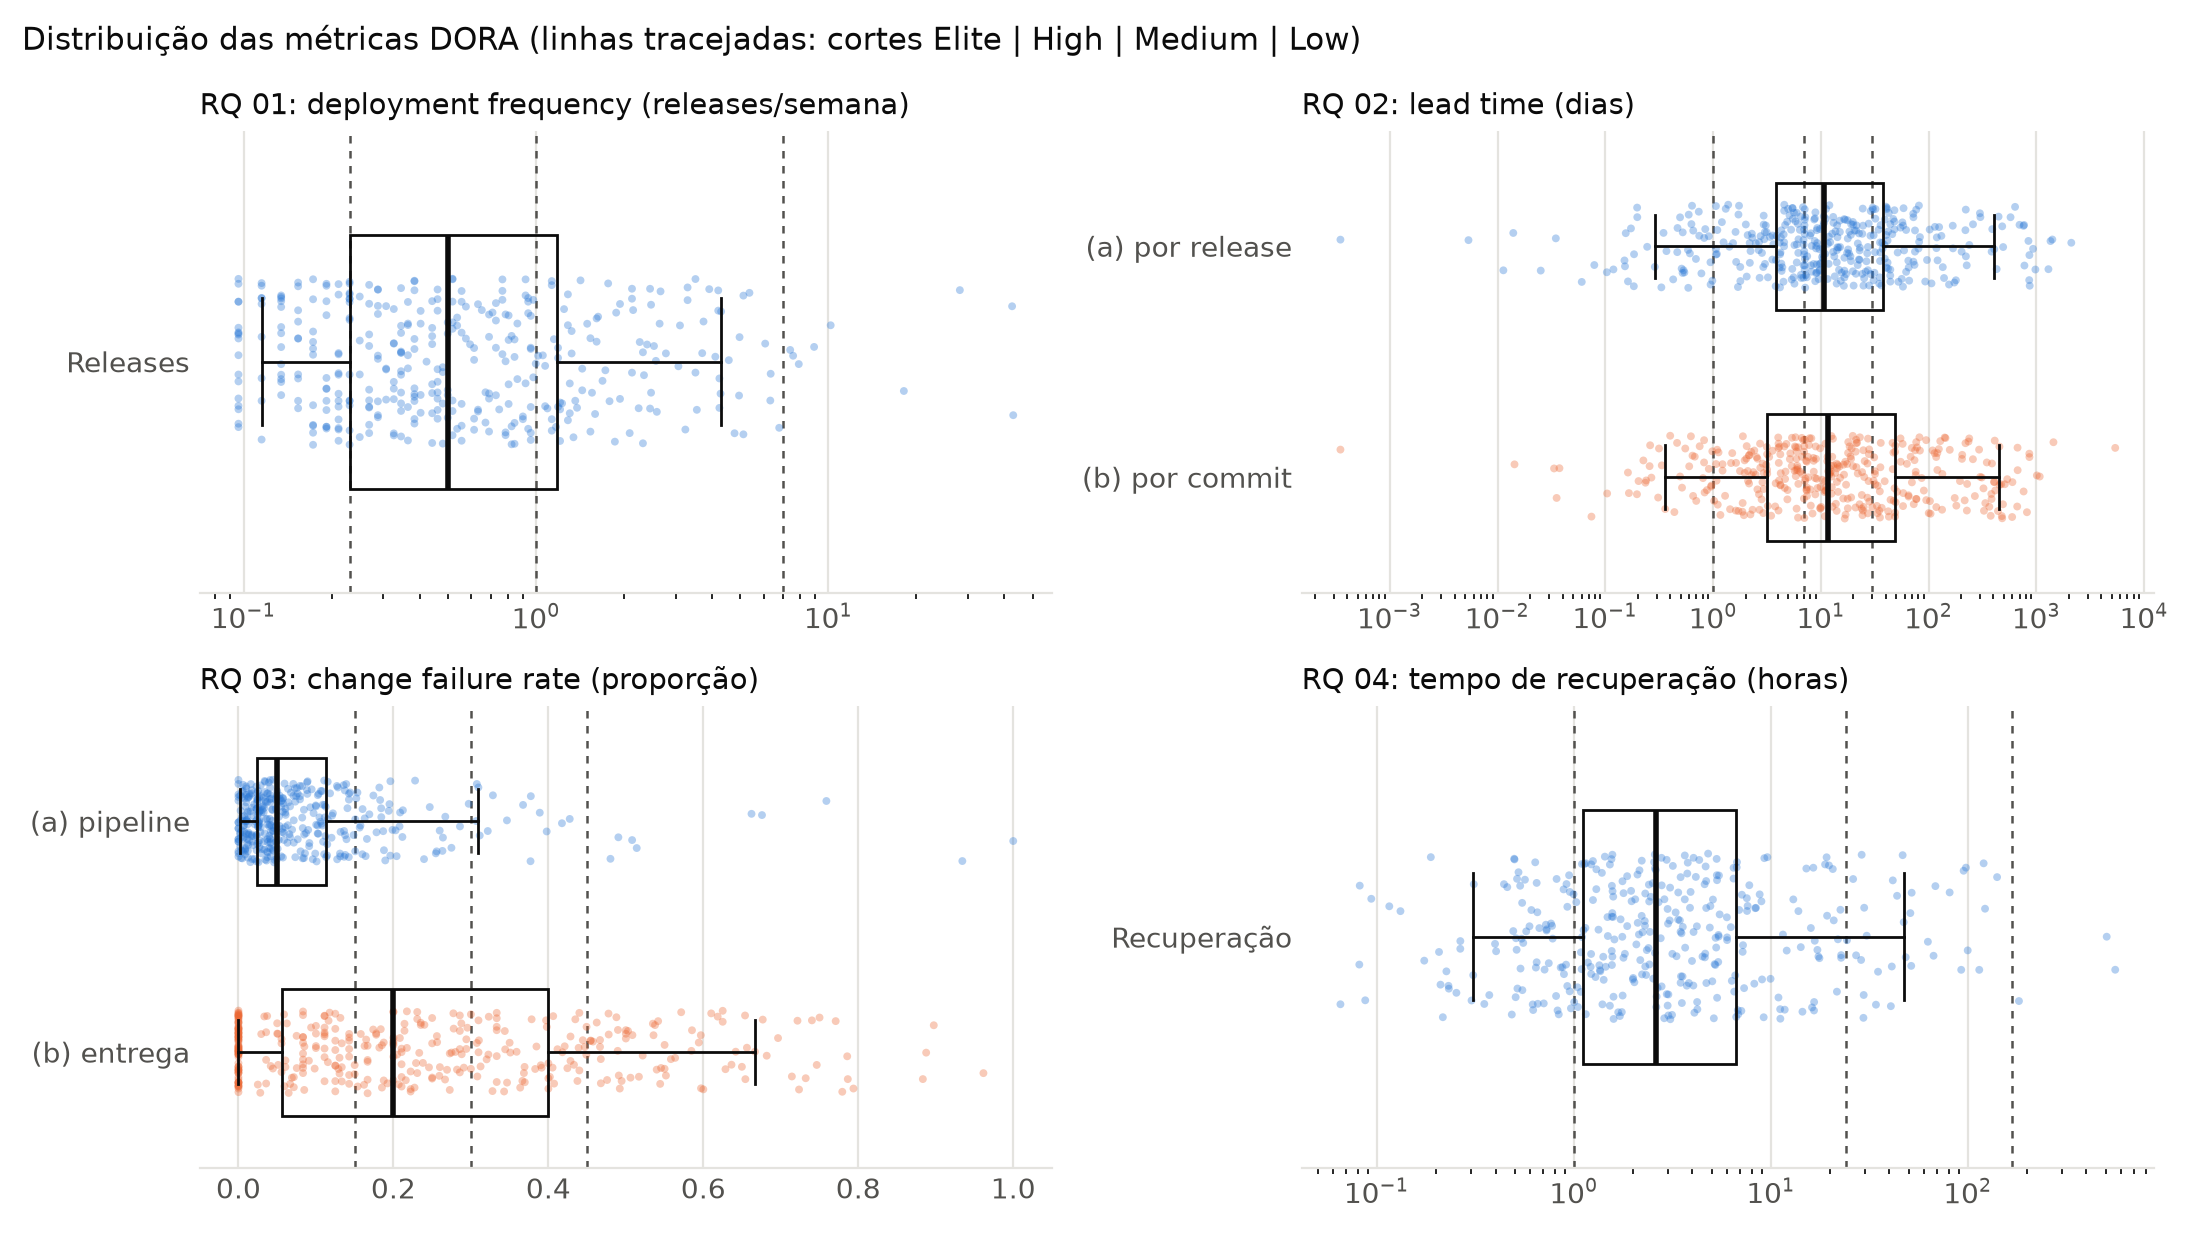
\includegraphics[width=.95\textwidth]{figuras/distribuicoes.png}
\caption{Distribuição das métricas das RQs 01 a 04. Caixas: Q1, mediana e Q3; bigodes: percentis 5 e 95; linhas tracejadas: cortes da classificação DORA.}
\label{fig:distribuicoes}
\end{figure}

\textbf{RQ 01.} O repositório típico publica 0,50 release por semana, uma a cada duas semanas (Tabela~\ref{tab:descritivas}). A distribuição tem cauda longa (Figura~\ref{fig:distribuicoes}): os 10\% mais ativos concentram 57,0\% das releases, e só 2,3\% dos repositórios são Elite.

\textbf{RQ 02.} As medianas das variantes são próximas (10,7 e 11,7 dias), mas elas divergem caso a caso. Dentro de uma release, a variante (a) é sempre a maior, porque usa o commit mais antigo, e ela supera a (b) em 60,6\% dos repositórios. No agregado, a (b) dá peso a cada commit, e por isso as releases grandes, que acumulam meses de trabalho, a puxam para cima: o percentil 90 é de 266 dias, contra 135 na (a).

\textbf{RQ 03.} O CFR (a) tem mediana de 4,9\%, e 82,5\% dos repositórios caem na faixa Elite: o CI do default branch roda depois do merge, quando as mudanças já passaram pelos testes do pull request. O CFR (b) tem mediana de 20,0\%, cerca de quatro vezes maior. As duas variantes quase não se correlacionam ($\rho = 0{,}147$), o que confirma que medem coisas diferentes.

\textbf{RQ 04.} A recuperação é rápida: mediana de 2,6 horas, e 90\% dos repositórios recuperam o pipeline em menos de um dia. Só 1,04\% dos episódios ficaram censurados, o que confirma a hipótese, mas em escala pequena.

\begin{figure}[ht]
\centering
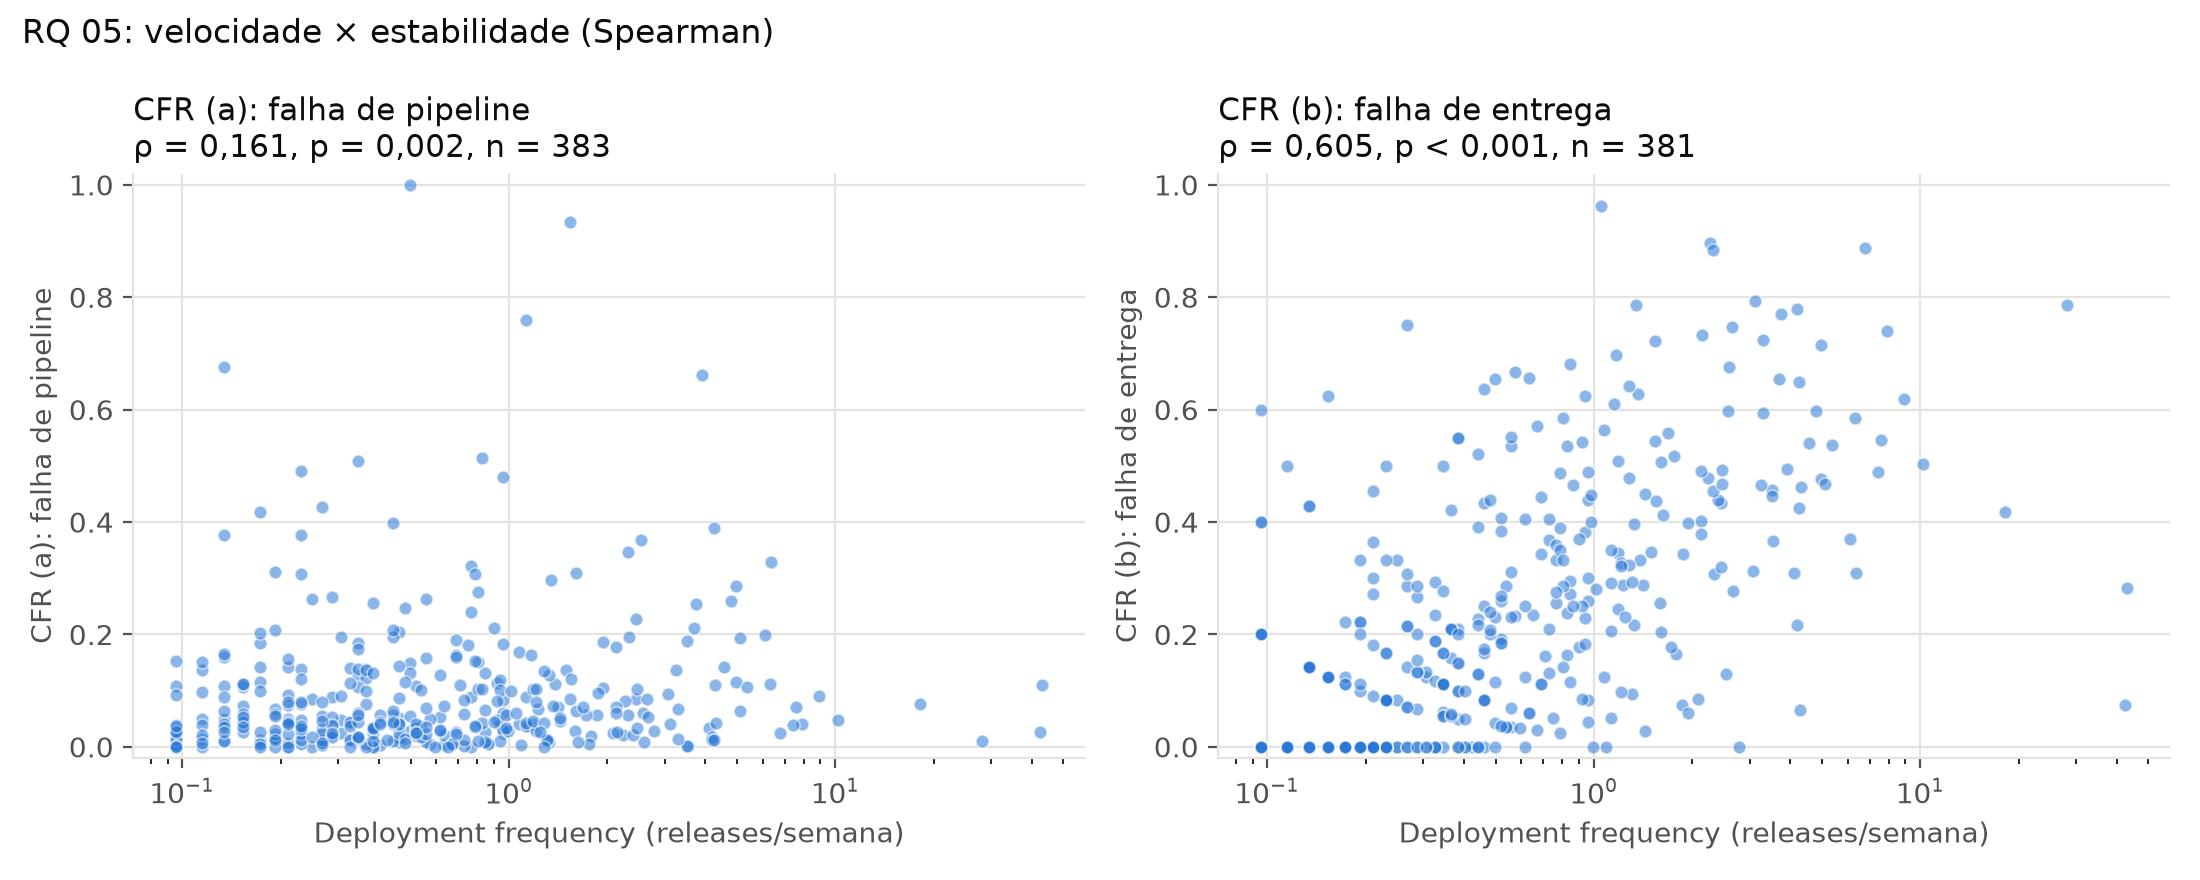
\includegraphics[width=.9\textwidth]{figuras/dispersao.png}
\caption{Deployment frequency (escala log) e CFR nas duas variantes.}
\label{fig:dispersao}
\end{figure}

\textbf{RQ 05.} A correlação entre frequência de deploy e CFR é positiva nas duas variantes, mas com intensidade bem diferente (Figura~\ref{fig:dispersao}): fraca com o CFR (a) ($\rho = 0{,}161$, $p = 0{,}002$, $n = 383$) e moderada com o CFR (b) ($\rho = 0{,}605$, $p < 0{,}001$, $n = 381$). Parte dessa relação vem da própria definição: uma release só falha se a correção sair em até 7 dias, e quem publica mais tem mais chances de cumprir essa condição.

\textbf{RQ 06.} Foram testados cinco fatores com as quatro métricas de C1, num total de 20 testes de Kruskal-Wallis corrigidos por Holm (Figura~\ref{fig:efeitos}), e seis foram significativos. A \textbf{idade} é o fator mais forte: os repositórios mais novos (Q1, menos de 2,6 anos) têm lead time mediano de 2,9 dias, contra 42,3 dias nos mais antigos (Q4), com $\varepsilon^2 = 0{,}317$ e Cliff's $\delta = 0{,}800$. Os mais novos também publicam mais e recuperam o pipeline mais rápido. Os \textbf{contribuidores} estão associados só ao lead time ($\varepsilon^2 = 0{,}151$), e a \textbf{linguagem}, à frequência e ao lead time, com o TypeScript à frente. A \textbf{popularidade} não tem associação com nenhuma métrica ($\varepsilon^2 \leq 0{,}018$), e o CFR (a) não difere entre os grupos de nenhum fator. O \textbf{tipo do projeto} também não teve diferença significativa, mas só cobre os 60 repositórios da amostra-ouro.

\begin{figure}[ht]
\centering
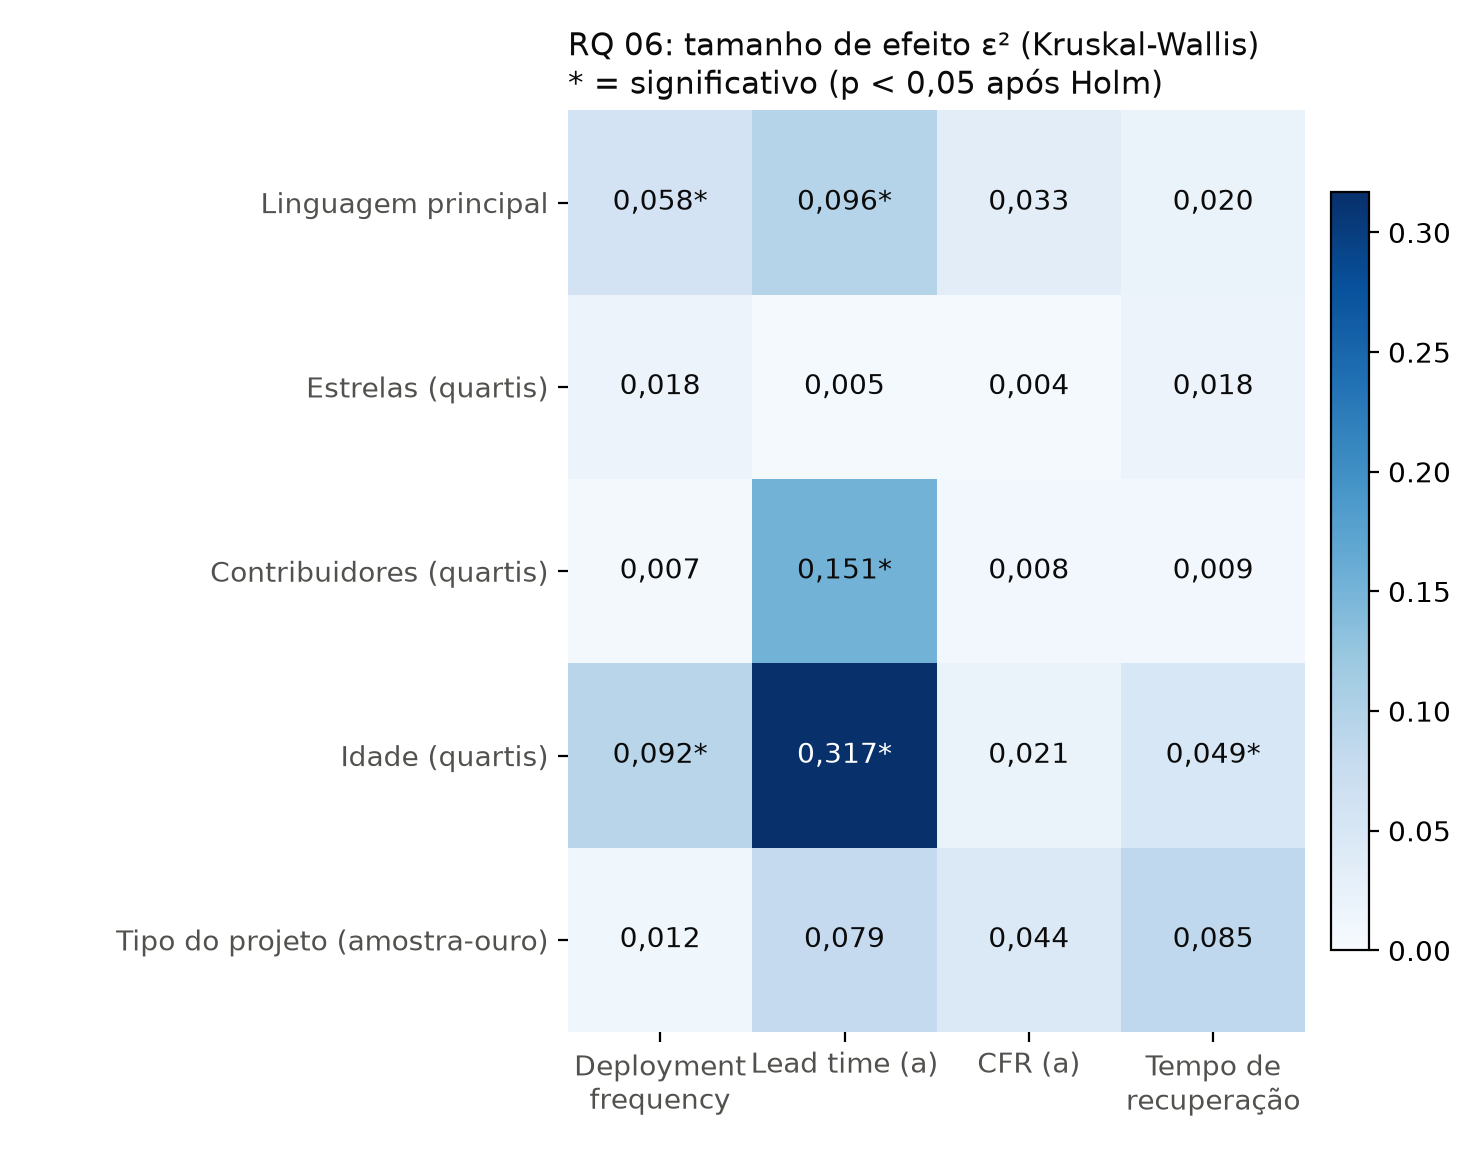
\includegraphics[width=.8\textwidth]{figuras/efeitos.png}
\caption{Tamanho de efeito $\varepsilon^2$ por fator e métrica (* = significativo após Holm).}
\label{fig:efeitos}
\end{figure}

\textbf{RQ 07.} Entre um quinto e quase um terço dos repositórios muda de categoria geral quando a definição muda (Tabela~\ref{tab:sensibilidade}), mas quase sempre para a faixa vizinha, por isso o kappa ponderado fica entre 0,518 e 0,700. A métrica mais frágil é o CFR: trocar o proxy de CI pelo de entrega muda a categoria de 60,4\% dos repositórios, com $\kappa = 0{,}033$, praticamente o acaso. A frequência é a mais estável. O kappa ponderado depende da ordem das categorias: sem o parâmetro \texttt{labels}, o \texttt{cohen\_kappa\_score} do scikit-learn as ordena alfabeticamente e daria 0,457, e não 0,553, para o lead time entre C1 e C2.

\begin{table}[ht]
\centering
\caption{Repositórios que mudam de categoria e kappa de Cohen ponderado entre combinações.}
\label{tab:sensibilidade}
\small
\begin{tabular}{lrrrrrr}
\hline
 & \multicolumn{2}{c}{C1 $\times$ C2} & \multicolumn{2}{c}{C1 $\times$ C3} & \multicolumn{2}{c}{C2 $\times$ C3} \\
Métrica & mudam & $\kappa$ & mudam & $\kappa$ & mudam & $\kappa$ \\
\hline
\textbf{Geral} & \textbf{29,8\%} & \textbf{0,518} & \textbf{20,9\%} & \textbf{0,700} & \textbf{26,0\%} & \textbf{0,590} \\
Deployment frequency & 11,7\% & 0,844 & 25,6\% & 0,644 & 14,1\% & 0,783 \\
Lead time & 43,9\% & 0,553 & 41,0\% & 0,590 & 11,2\% & 0,873 \\
CFR & 60,4\% & 0,033 & 0,0\% & 1,000 & 60,4\% & 0,033 \\
\hline
\end{tabular}
\end{table}

\textbf{RQ 08.} No repositório típico, metade das releases é corretiva: o rework rate tem mediana de 0,500 (IQR de 0,300 a 0,716), duas vezes e meia o CFR (b). As duas métricas estão moderadamente correlacionadas ($\rho = 0{,}446$), mas o rework rate é maior em 87,9\% dos repositórios. A diferença está no que cada uma conta. O CFR (b) atribui a falha à release quebrada e só considera correções em até 7 dias. O rework rate conta as próprias releases de correção, sem limite de tempo e sem censura.

\section{Discussão}

\begin{table}[ht]
\centering
\caption{Hipóteses e resultados.}
\label{tab:hipoteses}
\small
\begin{tabular}{lll}
\hline
RQ & Hipótese & Resultado \\
\hline
01 & frequências concentradas & confirmada (10\% concentram 57\% das releases) \\
02 & lead time (b) menor & parcial (vale em 61\% dos repositórios) \\
03 & proxies não equivalentes & confirmada ($\rho = 0{,}147$; $\kappa = 0{,}033$) \\
04 & há censura & confirmada, em escala pequena (1,0\%) \\
05 & relação fraca ou nula & depende do proxy ($\rho$ = 0,161 ou 0,605) \\
06 & quatro fatores associados & parcial (idade, contribuidores e linguagem; popularidade não) \\
07 & categorias mudam & confirmada (21\% a 30\%) \\
\hline
\end{tabular}
\end{table}

\textbf{O que surpreendeu.} O grupo esperava que projetos mais populares tivessem processos de entrega mais maduros, mas as estrelas não explicam nada, e a idade explica muito. Uma explicação provável é o ciclo de vida: projetos novos publicam versões pequenas e frequentes, e projetos antigos acumulam semanas de mudanças em cada release. A idade, porém, anda junto com o número de contribuidores ($\rho = 0{,}56$) e com a linguagem, e os testes de um fator por vez não separam esses efeitos.

\textbf{As conclusões são robustas?} A frequência de deploy e o tempo de recuperação são robustos às definições. O lead time é moderadamente robusto: as categorias mudam, mas para faixas vizinhas, e a associação com a idade aparece nas duas variantes. Tudo o que envolve o CFR, não. A categoria muda em 60\% dos repositórios, a RQ 05 passa de ``relação fraca'' a ``moderada'' conforme o proxy, e a idade só tem efeito sobre o CFR (b) ($\varepsilon^2 = 0{,}113$, numa análise exploratória). Com estes proxies, os dados não sustentam a tese do DORA de que velocidade e estabilidade não competem. Mais do que isso, mostram que nenhuma afirmação sobre estabilidade em open source pode ser feita sem dizer qual proxy de falha foi usado.

\section{Ameaças à validade}

Seguindo \cite{wohlin2012}:

\textbf{Construto.} Release não é deploy: uma biblioteca que publica uma release não coloca nada em produção, e monorepos com uma release por pacote, como o \texttt{expo/expo}, inflam a frequência. Falha de CI não é falha em produção. A heurística de release corretiva erra cerca de um quarto das releases que marca (precisão 0,728), e o próprio conceito é ambíguo para humanos ($\kappa = 0{,}477$). Nos 78 casos divergentes de release corretiva, o consenso equivale ao julgamento de um só avaliador. O \texttt{commit.author.date} pode anteceder em muito a entrada do commit no default branch.

\textbf{Interna.} Idade, contribuidores e linguagem são correlacionados. O CFR (b) depende da frequência por construção. A heurística foi escolhida e avaliada na mesma amostra, o que a verificação em metades aleatórias atenua, mas não elimina. Os cortes de 1.000 runs por mês e de 2.000 commits por release afetam, respectivamente, o CFR (a) e a recuperação em 96 repositórios, e o lead time (b) em 2,6\% das releases.

\textbf{Externa.} A amostra só tem projetos populares, com Actions e que publicam releases. Os resultados não valem para projetos pequenos, para projetos que versionam só por tags nem para equipes corporativas. Além disso, foram usadas uma única janela e uma única plataforma.

\textbf{Conclusão.} Os muitos testes da RQ 06 foram corrigidos por Holm e acompanhados de tamanho de efeito. O tipo do projeto tem poucos repositórios por grupo e pouco poder estatístico. Com $n \approx 380$, correlações fracas já são significativas, por isso a interpretação se baseia no tamanho de $\rho$. O paradoxo do kappa exige reportar também a concordância bruta.

\section{Replicação cruzada}

% A preencher na entrega final: pipeline replicado, problemas encontrados, comparação com o
% CSV original (diferença relativa por métrica e % de repositórios com a mesma classificação)
% e Issues abertas e recebidas.
\textit{A preencher na entrega final.}

\section{Disponibilidade}

Código, dados, resultados e protocolo de rotulagem: \url{https://github.com/FelipeVieir4/lab03-medicao-experimentacao-software-}. GitHub Projects: \textless preencher\textgreater.

\begin{thebibliography}{9}

\bibitem{dora}
DORA. \textit{DORA's software delivery metrics: the four keys}. Disponível em \url{https://dora.dev/guides/dora-metrics-four-keys/}.

\bibitem{feinstein1990}
Feinstein, A. R.; Cicchetti, D. V. (1990). High agreement but low kappa: I. The problems of two paradoxes. \textit{Journal of Clinical Epidemiology}, 43(6):543--549.

\bibitem{forsgren2018}
Forsgren, N.; Humble, J.; Kim, G. (2018). \textit{Accelerate: The Science of Lean Software and DevOps}. IT Revolution.

\bibitem{landis1977}
Landis, J. R.; Koch, G. G. (1977). The measurement of observer agreement for categorical data. \textit{Biometrics}, 33(1):159--174.

\bibitem{wohlin2012}
Wohlin, C. et al. (2012). \textit{Experimentation in Software Engineering}. Springer.

\end{thebibliography}

\end{document}
